% ============================================================
\chapter{財務と ESG}\label{ch:esg}

財務のデータ（割安さ、収益性、投資）と ESG の点数は、銘柄の性質を表す情報である。BL では、こうした性質を (1) ファクターのプレミアムと露出からビューを作る、(2) 均衡や事前分布の目標を調整する、(3) 共分散やリスクの側を調整する、のいずれかで入れられる。この章では、Fama--French のファクターへのビューを数値例で示し、ESG については、調査メモの「共分散を ESG の点数で膨らませる」方法を検討する。

\section{ファクターのプレミアムからビューを作る}

Fama と French（1993、2015）のファクターモデルは、株式のリターンを、市場、規模（SMB）、割安さ（HML）、収益性（RMW）、投資（CMA）のファクターで説明する。これにモメンタム（Carhart 1997）を加えた 6 ファクターがよく使われる。

ファクターを使ってビューを作る方法は 2 つある。

\begin{enumerate}
\item \textbf{銘柄ごとの絶対ビュー}：露出 $B$ とファクターのプレミアムの見込み $\hat\mu_f$ から、$Q=B\hat\mu_f$ を作る。調査メモの「Fama--French の回帰の結果をビューにする」はこの形である。ただし、ファクターの見込みが外れると全銘柄の予想が同じ向きに外れるので、$\Omega$ を対角にしてはいけない（外れの共分散は $B\,\Var(\hat\mu_f)\,B\T$）。
\item \textbf{ファクターへのビュー}：ファクターのプレミアム $\mu_f$ に事前分布を置き、ファクターへのビューで更新する（\chapref{ch:shape}、Kolm and Ritter 2017）。外れの相関が自然に入る。
\end{enumerate}

ここでは 2 番目の方法を、本プロジェクトのセクター ETF（データが長くそろう 9 セクター）と、Kenneth French のデータの 6 ファクターで試す。

\subsection*{設定}

\begin{itemize}
\item \textbf{露出 $B$}：セクター ETF の月次の超過リターンを、6 ファクターに回帰して推定する（2015 年 2 月〜2026 年 8 月の \V{fac.n} か月）。6 ファクターは、セクターの分散の平均 \V{fac.share}\% を説明する。
\item \textbf{事前分布}：ファクターのプレミアムの事前の平均 $\xi$ は、1963 年 7 月〜2014 年 12 月の \V{fac.Tlong} か月の平均（評価期間と重ならない）。モメンタムは年率 \V{fac.mom.prior}\% である。事前の不確かさは $V=F_{\mathrm{long}}/T_{\mathrm{eff}}$（$F_{\mathrm{long}}$ は同じ期間のファクターの共分散）とし、$T_{\mathrm{eff}}$ を変えて事前分布の強さを変える。
\item \textbf{ビュー}：「これからの 12 か月、モメンタムのプレミアムは 0 になる」（モメンタムの急落を心配する、という見方）。不確かさは、12 か月の平均の標準誤差 $\omega=F_{\mathrm{mom}}/12$ とした。
\end{itemize}

\begin{table}[htbp]
\centering
\caption{事前分布の強さ $T_{\mathrm{eff}}$ と、モメンタムへのビューの効き方（年率 \%）。右の 5 列は、ほかのファクターのプレミアムの事後の変化。$T_{\mathrm{eff}}=\V{fac.Tlong}$ は 1963〜2014 年の全データを信じる場合。}
\label{tab:fac-prior}
\tabin{fac_prior}
\end{table}

\tabref{tab:fac-prior} から分かることを挙げる。

\begin{itemize}
\item 事前分布を全データの長さ（$T_{\mathrm{eff}}=\V{fac.Tlong}$ か月）で信じると、12 か月分の見込みのビューの採用率は 1.9\% しかない。50 年分の平均は、1 年分の見込みでは動かない。$\tau\approx1/T$ の考え方（\chapref{ch:tau}）を、ファクターの単位で見たものである。
\item $T_{\mathrm{eff}}=120$（10 年分の確かさ）なら採用率は \V{fac.adopt120}\%、36 か月なら 25\% になる。ファクターのプレミアムは時代とともに変わるので、全データを信じすぎないほうがよい、という判断で $T_{\mathrm{eff}}$ を短くする。
\item モメンタムのプレミアムを下げるビューは、ほかのファクターのプレミアムも動かす。事前の不確かさ $V$ がファクターの共分散に比例しているため、モメンタムと負の相関を持つ市場やバリューのプレミアムが少し上がる。
\end{itemize}

\begin{table}[htbp]
\centering
\caption{$T_{\mathrm{eff}}=120$ のときの、セクターの期待超過リターン（年率 \%）。事前は $B\xi$、事後は $B\mu_f^{\mathrm{post}}$（ファクターで説明できない部分は 0 とした）。}
\label{tab:fac-assets}
\tabin{fac_assets}
\end{table}

\tabref{tab:fac-assets} のとおり、モメンタムへの露出が負のエネルギー（モメンタムの $\beta$ が $-0.36$）は期待リターンが上がり、露出が正の公益は下がる。1 つのファクターへのビューが、露出を通じて全セクターに一貫した形で効く。変化の大きさは年率で 0.5\% 以下と小さいが、これは事前分布が強く、ビューの採用率が 9\% 程度だからである。

\begin{tipbox}[コツ：ファクターへのビュー]
\begin{enumerate}
\item ファクターのプレミアムには長い歴史があるので、事前分布をデータで作れる。ただし、全データをそのまま信じると、どんなビューもほとんど効かない。プレミアムが時代とともに変わることを考えて、事前分布の強さ（$T_{\mathrm{eff}}$）を決める。
\item ビューの不確かさは、ビューの期間の平均の標準誤差（$F/\text{月数}$）が出発点になる。
\item 銘柄ごとのビュー $Q=B\hat\mu_f$ にするなら、外れの共分散 $B\,\Var(\hat\mu_f)B\T$ を $\Omega$ に入れる。対角にしない。
\end{enumerate}
\end{tipbox}

\section{割安さ・収益性などの銘柄の指標}

本プロジェクトは、銘柄ごとの PER、PBR、ROE、売上の伸びなどの指標を DB に持っている（『総合報告書』の「銘柄の指標」の章）。こうした指標をビューにするには、次の手順が素直である。

\begin{enumerate}
\item 指標をセクターの中で順位にし、点数 $z$ に直す（業種によって意味が変わる指標は、業種の中で比べる）。
\item 過去のデータで、点数と翌月のリターンの IC を測る。
\item Grinold の式 $\alpha=\IC\cdot\sigma\cdot z$ で期待リターンのずれにし、$\Omega$ は $\omega=\sigma^2(1/\IC^2-1)$（市場版）、または $\Omega\propto\Sigma$ で採用率 $\IC^2$ にする（\chapref{ch:accuracy}）。
\end{enumerate}

LLM に指標を渡して予想させても、予想はほとんど変わらなかった（『総合報告書』実験 D）。指標をビューにするなら、LLM を通さず、統計的な点数として直接入れるほうが、当たり具合を測りやすい。

\subsection*{本プロジェクトの指標の当たり具合}

本プロジェクトの DB の銘柄の指標（\code{stock\_metrics}）で、各月末の指標の順位と、翌月のリターンの順位相関（IC）を測った。期間は \V{tic.start}〜\V{tic.end} の月末、対象はその時点の \SP{} の構成銘柄である。割安さは、PER・PBR が低いほど高い点数になる向きにした。

\begin{table}[htbp]
\centering
\caption{銘柄の指標の IC（翌月のリターンとの順位相関の、月ごとの値の平均）。採用率は $\IC^2$、右端は Grinold の式で、月次の標準偏差 8\% の銘柄の点数が 1 標準偏差離れているときの期待リターンのずれ（月次 \%）。}
\label{tab:stock-ic}
\tabin{stock_ic}
\end{table}

\begin{figure}[htbp]
\centering
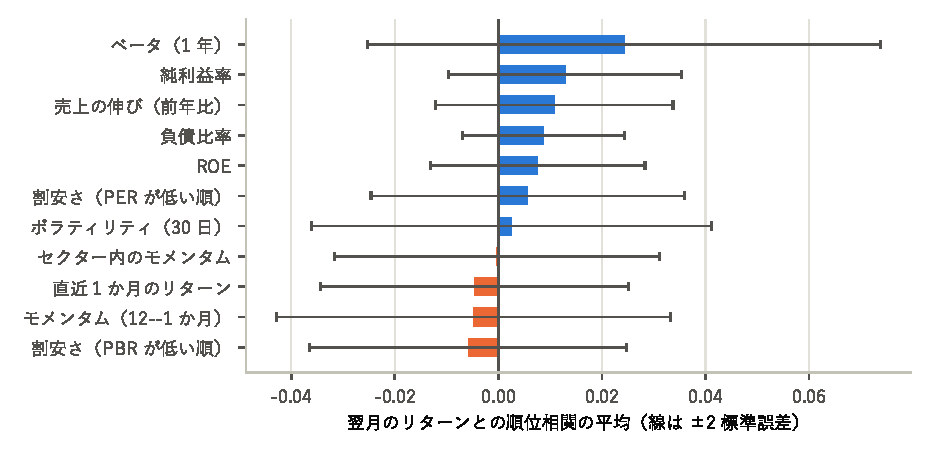
\includegraphics[width=0.9\linewidth]{fig_stock_ic.pdf}
\caption{銘柄の指標の IC の平均と、その ±2 標準誤差。}
\label{fig:stock-ic}
\end{figure}

\tabref{tab:stock-ic} と\figref{fig:stock-ic} のとおり、どの指標も IC の平均は絶対値で 0.025 以下で、$t$ 値が 2 を超えるものはなかった。いちばん大きいのはベータ（\V{tic.beta_1y.mean}、$t$ 値 \V{tic.beta_1y.t}）で、上昇相場の多かった期間に、市場に敏感な銘柄が少し勝ったことを表しているにすぎない。12--1 か月のモメンタムは \V{tic.momentum_12m.mean}、割安さ（PER）は \V{tic.pe_trailing.mean} で、この期間の大型株では、よく知られたファクターも単独ではほとんど効いていない。

この表は、BL のビューの大きさについて、はっきりした教訓を与える。単独の指標の IC が 0.01 程度なら、採用率は 0.01\% のオーダーで、期待リターンはほとんど動かすべきでない。指標を組み合わせて IC を上げるか、効く局面を見分けられない限り、「指標を見て期待リターンを大きく動かす」のは、当たり具合に見合わない。逆に、本プロジェクトの LLM の予想の IC（30 か月で 0.05 程度）は、この表のどの指標より大きい。ただし期間が短く、偶然と区別できない（\chapref{ch:project}）。

\section{ESG を BL に入れる方法}

ESG の点数は、期待リターンの情報か、リスクの情報か、それとも投資家の好み（制約）か。答えによって、入れ方が変わる。

\begin{description}[leftmargin=2em,style=nextline]
\item[好み・制約として] Pedersen、Fitzgibbons、Pomorski（2021）は、ESG を気にする投資家の最適な比率を「ESG 効率的フロンティア」で表した。ESG の点数を、ポートフォリオの平均の ESG の点数の下限などの制約として最適化に入れるのが、いちばん素直である。
\item[期待リターンの目標として] Alpern と Rachev（2025）は、ESG の点数を、期待リターンの Stein 型の縮小推定の目標として使う（$m_i=(1-\lambda)\mu_i+\lambda\xi_i$、$\xi_i$ は ESG の点数）。さらに、均衡の比率を、ダウ平均の比率と ESG の点数に比例する比率の混合 $w_{\mathrm{eq}}=(1-\lambda)w_C+\lambda w_\xi$ にする。リスクは、正規逆ガウス分布（NIG）の多変量版で CVaR を測る。2017〜2021 年のダウ平均の 28 銘柄で、回転率に罰則を付けた戦略のいくつかが年率 40〜45\% になったと報告しているが、多くの組み合わせを試した結果で、標本外の検証は ESG のデータが短いためにできていないと著者自身が述べている。
\item[共分散の構造として] Zuber（2017）の修士論文は、BL の共分散の構造を変えて、ESG の点数に応じて比率を動かす方法を提案している。
\end{description}

\section{共分散を ESG で膨らませる案}\label{sec:esg-penalty}

調査メモは、ESG の点数（0〜1、1 が最高）を使って、共分散を
\begin{equation}
\tilde\Sigma_{ij}=\Sigma_{ij}\sqrt{(2-\mathrm{ESG}_i)(2-\mathrm{ESG}_j)}
\label{eq:esg-penalty}
\end{equation}
と膨らませ、BL の $\Sigma$ に使う方法を紹介している。点数が 1 の銘柄はそのまま、0 の銘柄は分散が 2 倍になる。この資料では、この式を提案した論文を見つけられなかった（\appref{app:check}）。ここでは、式の性質を確かめる。

式~\eqref{eq:esg-penalty} は、$D=\diag(\sqrt{2-\mathrm{ESG}_i})$ として $\tilde\Sigma=D\Sigma D$ と書ける。各銘柄の標準偏差を $\sqrt{2-\mathrm{ESG}_i}$ 倍にし、相関は変えない、という操作である。

\subsection*{均衡と最適化で同じ $\tilde\Sigma$ を使うと、何も変わらない}

BL の手順どおりに、均衡リターンも $\tilde\Pi=\delta\tilde\Sigma\wmkt$ で作り直すと、ビューがないときの比率は $(\delta\tilde\Sigma)^{-1}\tilde\Pi=\wmkt$ で、時価総額の比率のままである。\chapref{ch:prior} で見たとおり、$\Sigma$ に何をしても、均衡と最適化で同じものを使う限り、出発点の比率は変わらない。調査メモの「最適化はボラティリティの制約を避けるために低 ESG の銘柄の比率を自動的に減らす」は、この場合には起きない。

\subsection*{均衡を元の $\Sigma$ のままにすると、比率が動く}

均衡リターンを元の $\Sigma$ で作り（$\Pi=\delta\Sigma\wmkt$）、最適化だけを $\tilde\Sigma$ で行うと、比率は動く。これは、「ESG の低い銘柄は、市場が思っているより危ない」という見方を入れたことになる。

\begin{table}[htbp]
\centering
\caption{4 資産の例（標準偏差 20〜30\%、相関 0.5、$\delta=2.5$）。(1) 均衡も最適化も $\tilde\Sigma$、(2) 均衡は $\Sigma$、最適化は $\tilde\Sigma$（空売りなし・全額投資）。採用率は、各資産に絶対ビューを 1 つずつ置き、$\omega=0.04^2$、$\tau=0.05$ で固定したときの 1 資産あたりの値。右端は Alpern--Rachev の比率の混合（$\lambda=0.25$）。}
\label{tab:esg}
\tabin{esg}
\end{table}

\tabref{tab:esg} の (1) の列は時価総額の比率と一致し（差は最大 \V{esg.w1diff}\%）、(2) の列では、ESG の低い資産 D の比率が 0 になり、高い資産 A が増える。

\subsection*{ビューの採用率は、ESG の低い銘柄で上がる}

もう 1 つ、意図と逆の効果がある。$\Omega$ を外から固定していると、$\tau\tilde\Sigma$ が大きくなった銘柄ほど、均衡の不確かさが大きくなり、ビューの採用率が上がる（\tabref{tab:esg} の採用率の 2 列）。ESG の低い銘柄 D では、採用率が 73.8\% から 84.2\% に上がる。「ESG の低い銘柄は危ないので控えめに」という意図に反して、その銘柄についてのビュー（強気でも弱気でも）を強く信じることになる。

\begin{tipbox}[コツ：ESG を入れるとき]
\begin{enumerate}
\item ESG を共分散で表すなら、均衡を作る $\Sigma$ と最適化の $\Sigma$ のどちらに入れるのかをはっきりさせる。両方に入れると何も変わらない。
\item $\Omega$ を固定したまま共分散を膨らませると、その銘柄のビューの採用率が上がる。意図と逆になりうる。
\item ESG が投資家の好みなら、制約（ポートフォリオの平均の点数の下限、除外）で入れるのが素直である。期待リターンの情報だと考えるなら、ビューや均衡の目標として入れ、当たり具合を確かめる。
\end{enumerate}
\end{tipbox}

\begin{keybox}[この章のまとめ]
\begin{itemize}
\item ファクターへのビューは、露出を通じて全資産に一貫して効き、外れの相関も自然に入る。事前分布を長いデータで信じすぎると、ビューはほとんど効かない。
\item 銘柄の指標は、IC を測ってから Grinold の式で期待リターンに直すのが素直である。
\item 共分散を ESG で膨らませる案は、均衡と最適化で同じ共分散を使うと効かず、均衡を元のままにすると比率が動く。$\Omega$ を固定していると、ESG の低い銘柄のビューを強く信じる方向に働く。
\end{itemize}
\end{keybox}
